\chapter{Projekt i implementacja systemu}
\label{sec:implementacja-systemu}
W rozdziale tym opisano implementację systemu zaprojektowaną przy użyciu technologii opisanych w rozdziale \ref{chap:technologie}. Zdefinowano wymagania, jakie system ma spełniać, wraz z przedstawieniem jego projektu oraz architektury. Ponadto ukazano funkcje systemu z perspektywy użytkownika oraz zilustrowano przykładowe użycie oprogramowania. Na samym końcu przedstawiono szczegóły implementacyjne systemu, w tym uzasadnienie wyboru wykorzystanej architektury. 

\section{Wymagania funkcjonalne i założenia systemowe}
Projektowany system będzie służył synchronizacji różnych wymagań funkcjonalnych opisanych w niniejszym rozdziale. Będzie on wykonany w postaci oprogramowania. 
Oprogramowanie będzie wytworzone w formie aplikacji desktopowej, dostępnej na system operacyjny Windows 11. Aplikacja ta musi posiadać graficzny interfejs użytkownika (GUI) składający się z panelu sterującego oraz wyświetlacza. 
Oprogramowanie ma obługiwać jedną z dostępnych (niewykorzystywanych przez inne procesy) kamer podłączonych do komputera. Lista dostępnych kamer jest określana jednorazowo przed pojawieniem się GUI na ekranie. Dlatego w przypadku chęci użycia kamery podłączonej w trakcie wykonywania programu należy zamknąć aplikację (panel sterowania GUI) i uruchomić ją ponownie.

Na podstawie powyższych założeń, kolejne wymagania fukncjonalne można podzielić na dwa bloki: pierwszy (logiczny), drugi (wpływający na stan GUI). Na bazie pierwszego bloku system realizuje następujące funkcje:
\begin{itemize}
    \item Pobiera klatki obrazu z kamery.
    \item Zmniejsza rozmiar klatki, jeżeli jest on większy niż ekran monitora komputera.
    \item Wykrywa obiekty na podanej klatce obrazu.
    \item Przygotowuję klatkę obrazu do wyświetlenia -- wizuallizuje lokalizację obiektów bazując na wynikach detekcji, jeżeli znajdują się w nich wykrycia.
    \item Alarmuje dźwiękowo użytkownika, jeżeli obiekty zostały wykryte.
    \item Synchronizuje wyżej wypunktowane funkcje.
\end{itemize}

Na bazie drugiego bloku system:
\begin{itemize}
        \item Wyświetla przygotowane klatki obrazu w wyświetlaczu GUI.
        \item Umożliwia użytkownikowi wyłączenia źródła wideo (wyłączenia wyświetlacza) w panelu sterowania GUI.
        \item Umożliwia użytkownikowi ustawienie progu ufności detekcji (próg ufności opisany w rozdziale \ref{chap:wprowadzenie-yolo_interjes}) obiektów w panelu sterowania GUI.
        \item Umożliwia użytkownikowi ustawienie wykrywanych klas obiektów ze zdefiniowanego zbioru klas w panelu sterowania GUI.
        \item Umożliwia użytkownikowi wybór kamery jako źródło wideo z dostępnych kamer wejściowych w panelu sterowania GUI.
        \item Generuje listę dostępnych kamer przed wyświetleniem GUI.
\end{itemize}

System musi zorganizować funkcje w odpowiednie moduły i odpowiednio je synchronizować. Założoną architekturą systemu jest architektura wielowątkowa. 
\section{Architektura systemu}
\label{chap:architektura}
Najważniejsze elemety systemu można podzielić na dwa główne moduły: silnik przetwarzania wideo oraz interfejs użytkownika. 

Silnik przetwarzania wykonuje następujące zadania:
\begin{enumerate}
    \item Pobiera klatkę obrazu z kamery.
    \item Zmniejsza rozmiar klatki, jeżeli jest on większy niż ekran monitora komputera.
    \item Wykrywa obiekty na podanej klatce obrazu.
    \item Przygotowuję klatkę obrazu do wyświetlenia -- wizuallizuje lokalizację obiektów bazując na wynikach detekcji, jeżeli znajdują się w nich wykrycia.
    \item Alarmuje dźwiękowo użytkownika, jeżeli obiekty zostały wykryte.
    \item Przekazuje przygotowaną klatkę na wyjście modułu. 
\end{enumerate}

Operacja detekcji jest czasochłonna jak i również pobór klatki ze względu na ograniczenia sprzętowe kamery (FPS). Dlatego zamiast sekwencyjnej realizacji zadań silnika przetwarzania postanowiono podzielić go na dwa podmoduły oraz zrównoleglić ich wykonanie poprzez utworzenie wątku dla obu z nich. Zadania zawarte w każdym podmodule są wykonywane sekwencyjnie.

Pierwszy podmoduł realizuje w kolejności zadania nr 1 i nr 2, zaś moduł drugi -- w kolejności zadania od nr 3 do 6 włącznie. Przekazanie klatki pomiędzy wątkami (modułami) umożliwiono poprzez zastosowanie bufora (nazwanego buforem pośrednim) wraz z mechanizmami synchronizacji dostępu do niego (dalej opisanymi w szczegółach implementacyjncyh w rozdziale \ref{chap:szczegoly-implementacji}). Podmoduł pierwszy przekazuje klatkę do bufora przejściowego, natomiast podmoduł drugi czeka aż klatka ta zostanie przekazana po czym pobiera ją i czyści bufor przejściowy. 

Oprócz ustanowienia podmodułu drugiego oddzielnym wątkiem, podmoduł ten wywołuje wykonanie alarmu dźwiękowego (krok nr 4) w dodatkowym wątku. Bez użycia dodatkowego wątku dalsze kroki w podmodule zostałyby wykonane dopiero po zakończeniu alarmu -- po zakończeniu pliku dźwiękowego służącego jako alarm. Sekwencja podmodułu w większości przypadków wykonuję się szybciej niż odtworzenie całego pliku co w połączeniu z dodatkowym wątkiem może powodować nieprzyjemne dla użytkownika nałożenie się alarmów w tym samym czasie. Zastosowano więc mechanizm (opisany w rozdziale \ref{chap:szczegoly-implementacji}), który pozwala uniknąć wywołania alarmu, jeżeli poprzedni nie został zakończony.

Przechodząc do modułu interfejsu użytkownika, wykonuje on następujące funkcje systemu:
\begin{enumerate}
    \item Wyświetla przygotowane klatki obrazu w wyświetlaczu GUI.
    \item Umożliwia użytkownikowi wyłączenia źródła wideo (wyłączenia wyświetlacza) w panelu sterowania GUI.
    \item Umożliwia użytkownikowi wybór kamery jako źródło wideo z dostępnych kamer wejściowych w panelu sterowania GUI.
    \item Umożliwia użytkownikowi ustawienie progu ufności detekcji (próg ufności opisany w rozdziale \ref{chap:wprowadzenie-yolo_interjes}) obiektów w panelu sterowania GUI.
    \item Umożliwia użytkownikowi ustawienie wykrywanych klas obiektów ze zdefiniowanego zbioru klas w panelu sterowania GUI.
\end{enumerate}
Ważną informacją na temat funkcji od nr 2 do nr 4 są okoliczości ich użycia. Zainicjowane zostają jako efekt integracji użytkownika z panelem sterowania graficznego interfejsu użytkownika. Temat użycia GUI opisano w oddzielnym rozdziale \ref{chap:uzytkownik-gui}. 

Moduł interfejsu użytkownika również działa w oddzielnym wątku. Aby krok nr 1 był możliwy, wymagana jest komunikacja między modułem silnika (dokładniej podmodułem drugim).  
Należało tak jak w przypadku podmodułów silnika przetwarzania wideo zaimplementować sposób przekazywania klatki. Również użyto do tego bufora (nazwanego buforem wyjściowym) z mechanizmem synchronizacji dostępu. W tym wypadku oprócz klatki przesyłana jest również informacja czy kamera dalej działa, co może być przydatną informacją w przypadku odłączenia kamery od komputera. W przeciweństwie do podmodułu drugiego silnika, strona pobierająca dane (moduł interfejsu) nie czeka aż bufor jest pełny. Próba poboru klatki jest realizowana periodycznie. W sytuacji braku klatki periodyczny pobór jest kontuuowany. W sytacji kiedy przekazano informacje o niedziałaniu kamery, periodyczny pobór zostaje zakończony.

Periodyczny pobór jest wyłączony na starcie aplikacji i wywoływany jest dopiero poprzez ustawienie kamery funkcją nr 2. Pobór jest wyłączony również, w przypadku wykonania funkcji nr 3.

Oprócz wpływu na moduł interfejsu, funkcje nr 2 i 3 ingerują w zachowanie modułu silnika, więc komunikują się z nim. Domyślnie po włączeniu aplikacji wątki dla obu podmodułów silnika są utworzone lecz ich sekwencje nie rozpoczynają się dopóki nie zostanie wysłany sygnał. Sygnał jest informacją o tym, iż kamera została ustawiona i działa. Sygnał ten wysyłany jest za pomocą funkcji nr 3. Przeciwnie do nr 3, funkcja nr 2 usuwa źródło wideo, więc wstrzymuje dalsze powtórzenia obu sekwencji, tym samym oczekując na wznownienie wywołaniem funkcji nr 3.

Funkcje nr 4 i 5 ustawiają parametry modułu zawierającego model Yolov8n, który jest konieczny do przeprowadzenie kroku nr 3 silnika przetwarzania wideo. W module tym wykorzystywany jest interfejs opisany w rozdziale \ref{chap:wprowadzenie-yolo_interjes}. Funkcja nr 4 ustawia parametr \emph{conf}, zaś nr 5 -- parametr \emph{classes}. Funkcje te zmieniają jedynie te parametry, nie ingerując w działanie modułu silnika przetwarzania wideo, co pozwala kontuunacje całego procesu kończącego się wyświetleniem klatki na wyświetlaczu GUI.
Domyślne parametry detektora to 0.5 dla progu ufności i klasa człowiek jako klasy obiektów poddane detekcji.

Podsumowując, aplikacja wykorzystuje cztery wątki. Wyróżnić w niej można dwa główne moduły: moduł graficznego interfejsu użytkownika oraz moduł silnika przetwarzania wideo. Poprzez integracje użytkownika z panelem sterowania GUI moduł interfejsu kontroluje kluczowowe sekwencje, które dzięki skomunikowaniu wykonują cel niniejszego systemu -- alarmowanie audio-wizualne.  
\section{System z perspektywy użytkownika}
\label{chap:uzytkownik-gui}
Każdą funkcję realizowaną przez system można przypisać do kategorii logicznej lub kategorii zleconej. Kategoria zlecona zawiera wydarzenia, które użytkownik zainicjował poprzez integrację z panelem sterowania GUI. Kategoria logiczna zawiera funkcję, które mogą zostać wykonane, pośrednio lub bezpośrednio, jest następstwo wystąpienia wydarzeń.

Wyróżnia się trzy wydarzenia: zmiana parametru progu ufności detektora obiektów poprzez manipulację suwakiem (ang. \emph{slider}), ustawienie klas obiektów wykrywanych przez detektor poprzez zaznaczenie odpowiednich przycisków przy nazwach klas oraz wybór źródła wideo z menu --- może to być jedna z kamer podłączonych do komputera lub zapisany na dysku plik wideo albo opcja wyłączenia źródła wideo. Wygląd panelu sterowania zilustrowany jest na rysunku \ref{fig:panel-sterowania}. 
Uwaga: wybór pliku wideo jako źródła należy traktować jako dodatek. W dalszej części dokumentu kamera jest jedynym rozważanym źródłem wideo.   

\begin{figure}[H]
    \centering
    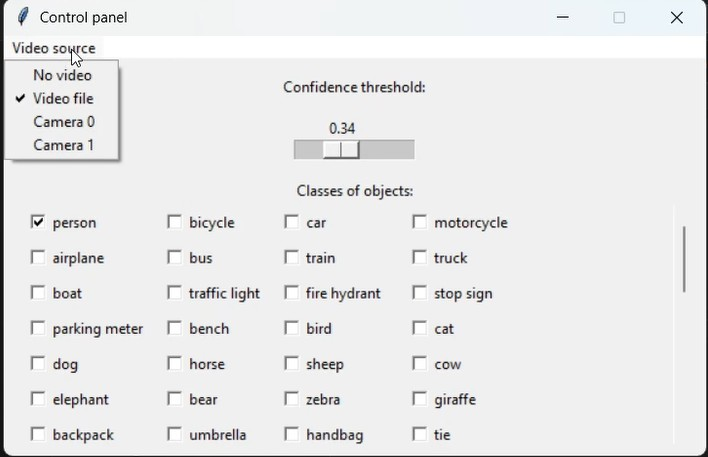
\includegraphics[width=\linewidth]{r_implementacja/panel_sterowania/panel.jpg}
    \caption{Panel sterowania graficznego interfejsu użytkownika.}
    \label{fig:panel-sterowania}
\end{figure}

Zmiana parametrów detektora może odbywać się w trakcie działania zadań dektecji obiektów. Po wystąpieniu wydarzania nowe wartości parametrów nadpisują ustawienia detektora i od tego momentu tryb inferencji będzie korzystać z nowych parametrów.

Wybranie źródła wideo skutkuje uruchomieniem ustalonej sekwencji funkcji logicznych. Sekwencja ta objemuję następujące kroki:
\begin{enumerate}
    \item Pobranie klatki obrazu z wybranego źródła wideo.
    \item Detekcja ustawionych klas obiektów na bazie pobranej klatki.
    \item Jeżeli wykryto choć jeden obiekt:
    \begin{enumerate}
        \item Przetworzenie klatki w celu narysowania wygenerowanych prostokątów ograniczających. 
        \item Alarmowanie w formie dźwiękowej. 
    \end{enumerate}
    \item Dostarczenie klatki do bufora.
    \item Pobranie klatki z bufora oraz wyświetlenie jej w wyświetlaczu GUI.
\end{enumerate} 
Sekwencja jest powtarzana do momentu zakończenia się pliku wideo lub wyłączenia bądź zmiany źródła wideo. 

Na podstawie funkcji systemu zobrazowano przykładowy scenariusz wykorzystania systemu przez użytkownika z kolejnymi krokami na ryskunkach \ref{fig:mockup-2}, \ref{fig:mockup-3}, \ref{fig:mockup-4}. Przykładowe użycie to nagranie sceny ze znajdującym się człowiekiem (twarz zamazano).

\begin{figure}[H]
    \centering
    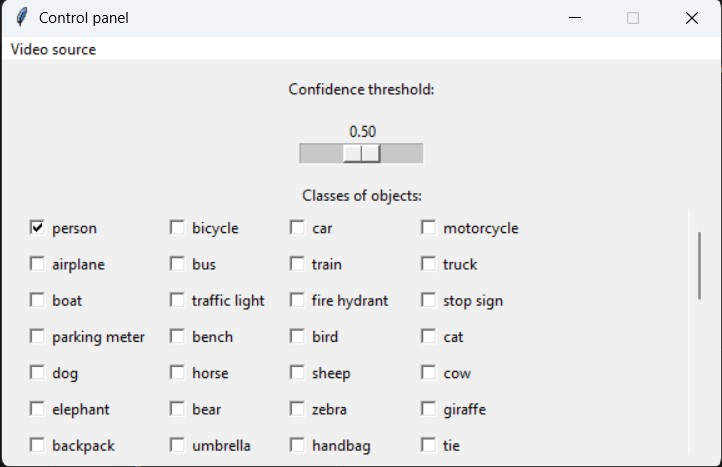
\includegraphics[width=\linewidth]{r_implementacja/panel_sterowania/panel_mockup.jpg}
    \caption{GUI w chwili uruchomienia aplikacji.}
    \label{fig:mockup-2}
\end{figure}

\begin{figure}[H]
    \centering
    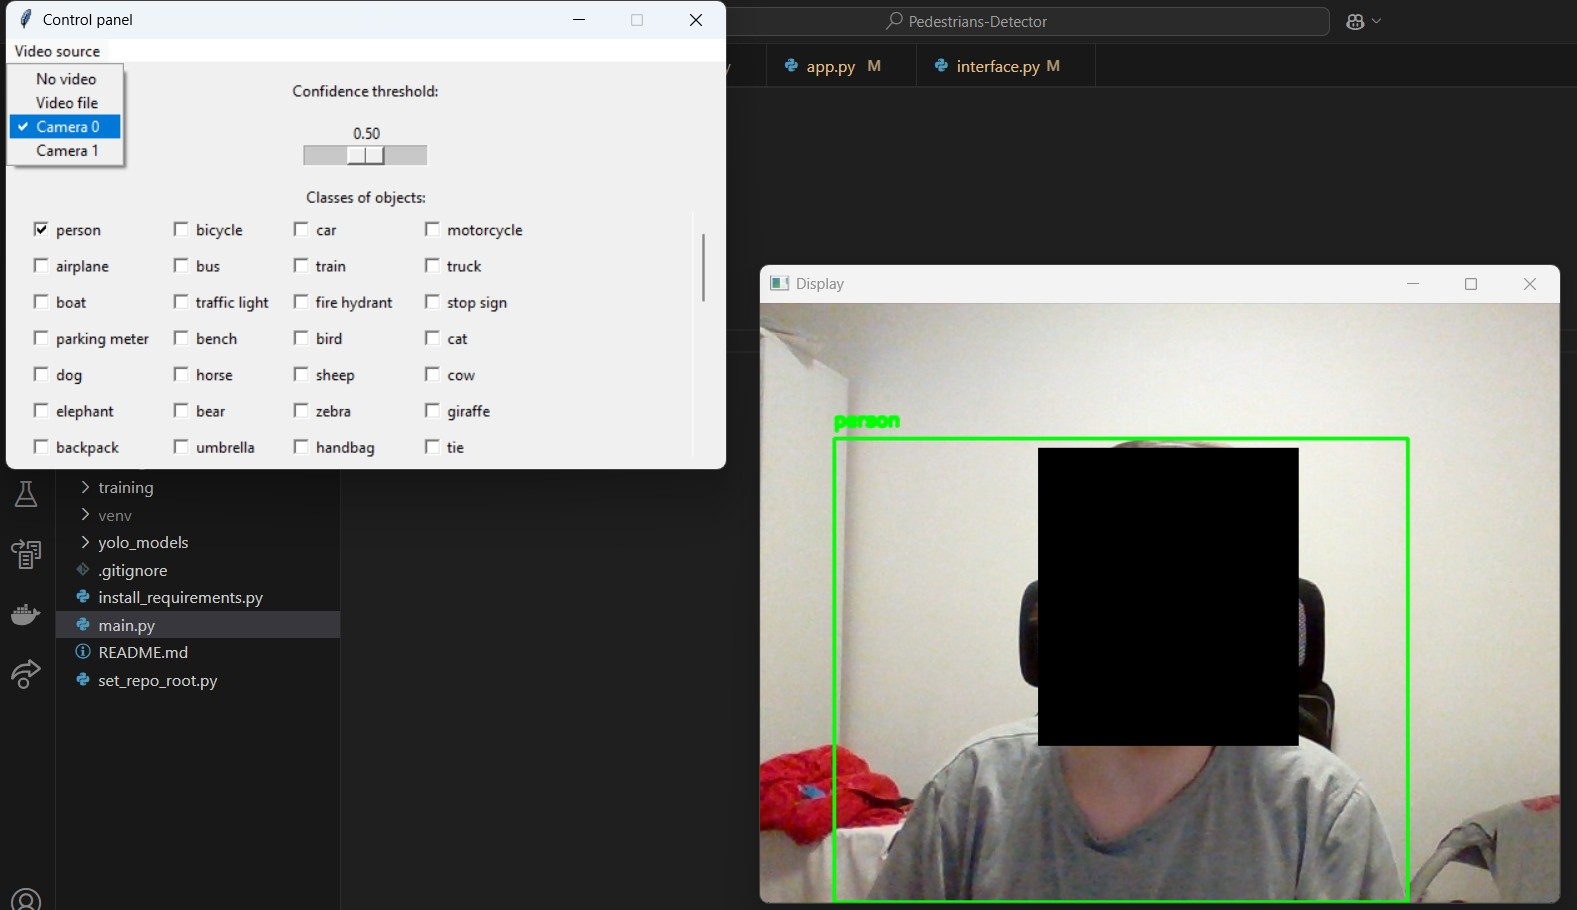
\includegraphics[width=\linewidth]{r_implementacja/panel_sterowania/camera_50.jpg}
    \caption{Uruchomienie wyświetlacza dla domyślnych parametrów detektora oraz kamery o indeksie 0.}
    \label{fig:mockup-3}
\end{figure}

\begin{figure}[H]
    \centering
    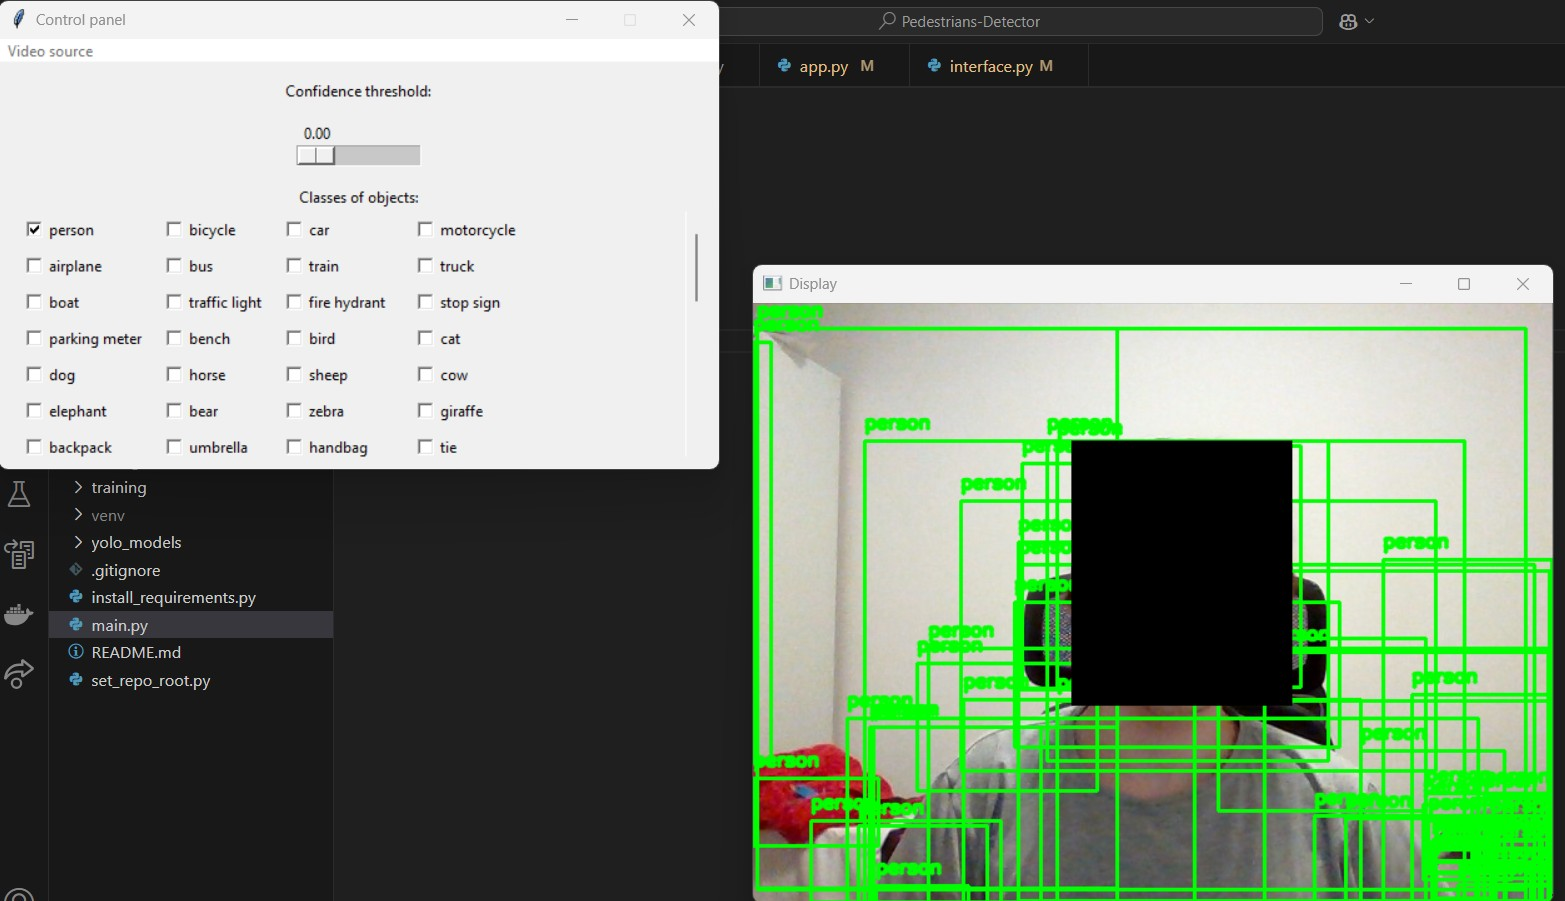
\includegraphics[width=\linewidth]{r_implementacja/panel_sterowania/camera_0.jpg}
    \caption{Zmiana progu ufności na 0.00.}
    \label{fig:mockup-4}
\end{figure}

\begin{figure}[H]
    \centering
    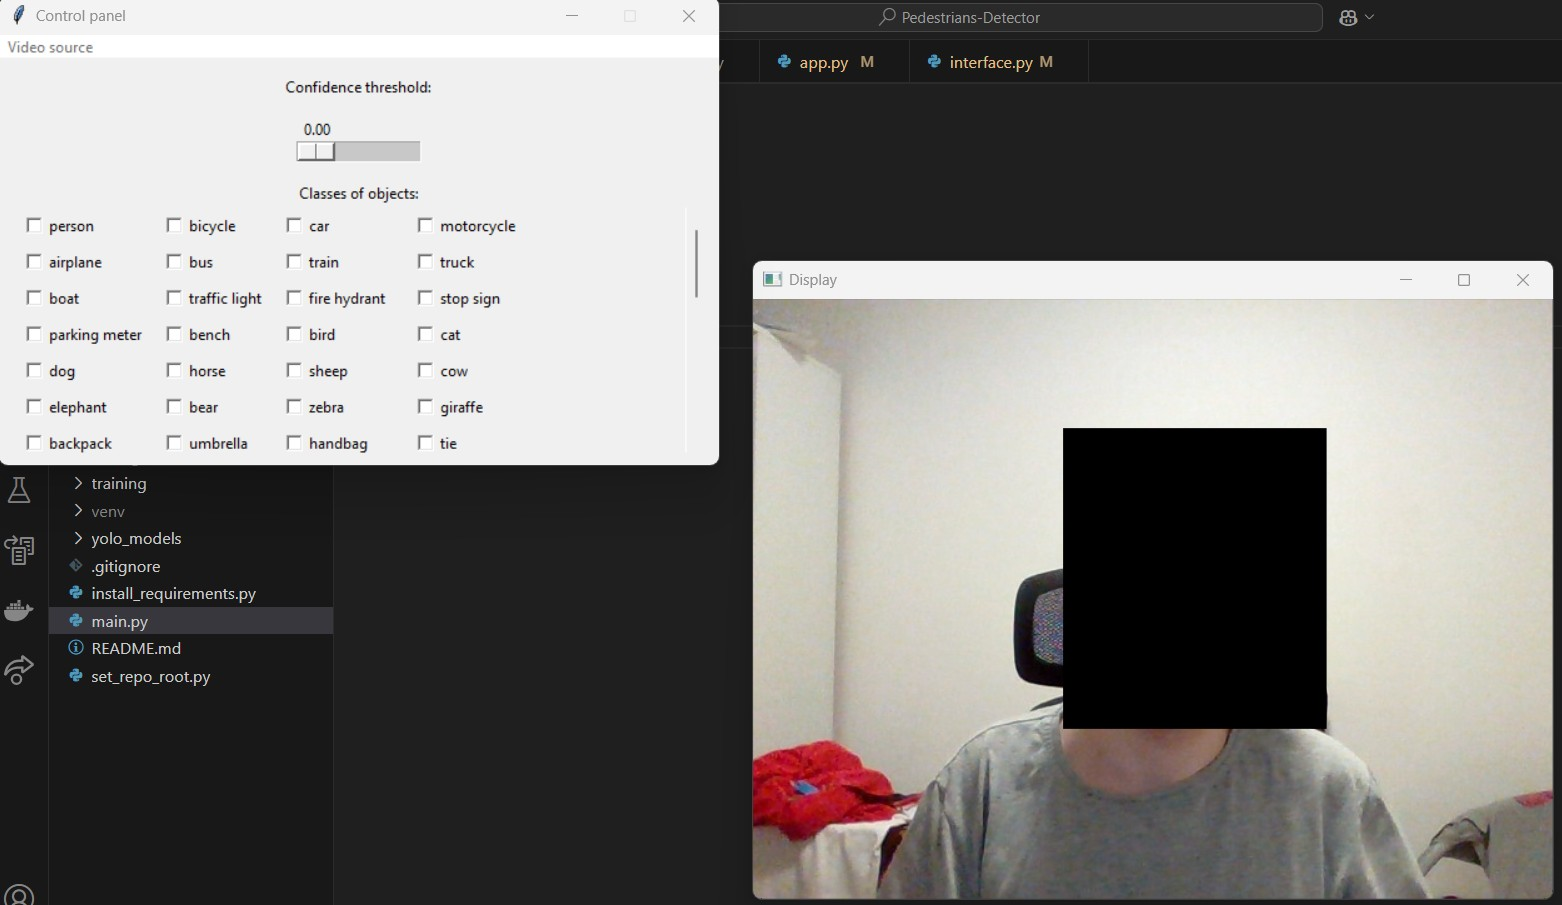
\includegraphics[width=\linewidth]{r_implementacja/panel_sterowania/camera_no_person.jpg}
    \caption{Usunięcie klasy człowiek z wykrywanych obiektów.}
    \label{fig:mockup-5}
\end{figure}

\section{Implementacja systemu na poziomie klas}
Oprogramowanie podzielono na sześć klas: \emph{App}, \emph{VideoCapture}, \emph{YoloInferenceConfig}, \emph{ImageProcessor}, \emph{VideoProcessingEngine} oraz \emph{GUI}.

\emph{App} jest punktem centralnym aplikacji. W tym miejscu rozpoczyna się program i tworzone są instancję pozostałych pięciu klas. Pierwszym zadaniem klasy jest utworzenie obiektów pozostałych klas. Następnie klasa ta służy jako interfejs do komunikacji między modułem interfejsu graficznego użytkownika (\emph{GUI}), a sekcją logiczną -- w tym do pobrania informacji o liście dostępnych kamer (\emph{VideoCapture}), ustawienia parametrów inferencji detektora (\emph{ImageProcessor}) oraz do komunikacji z silnikiem przetwarzania wideo (\emph{VideoProcessingEngine}).
Ponadto, klasa ta implementuje metodę, która uruchamia alarm dźwiękowy (\emph{{play\_audio\_alert}}). 
 
\emph{VideoCapture} służy do obługi źródła wideo. Klasa dostarcza kluczową metode, \emph{get\_frame}, której wywołanie zwraca informację o tym czy źródło wideo nadal jest dostępne oraz najnowszą dostępną klatkę z kamery. Ponadto warto wyróżnić metodę do pozyskania dostępnych do użycia kamer (\emph{get\_available\_sources}). Klasa ta zawiera również metody \emph{start\_capture} oraz \emph{end\_capture} odpowiedzialne kolejno za ustanowienie połączenia z podaną jako argument kamerą oraz zwolnienia tego połączenia. 

\emph{YoloInferenceConfig} jest to klasa, której głównym celem jest przechowywanie parametrów inferencji (progu ufności oraz wykrywanych klas) oraz dostarczenie metod do zmiany tych parametrów. Klase utworzono dla zachowania większej czytelności kodu w \emph{ImageProcessor}, dlatego też jest ona dziedziczona przez \emph{ImageProcessor} właśnie. W chwili uruchomienia aplikacji, klasa jest inicjalizowana domyślnymi parametrami: próg ufności równy $0.5$ oraz \emph{człowiek} jako wykrywana klasa. 

\emph{ImageProcessor} służy do przetwarzania oraz analizy obrazu. Kluczowe trzy metody to \emph{detect\_objects}, zwracająca liczbe wykrytych obiektów oraz wyniki detekcji na podstawie podanej klatki obrazu; \emph{visualize\_objects\_presence}, która na postawie w.w. wyników detekcji, rysuję prostokąty ograniczające dookoła wykrytych obiektów; \emph{fit\_frame\_into\_screen}, która zmniejsza rozmiar podanej klatki, jeżeli jest większa niż rozmiar ekranu monitora podłączonego do komputera.

\emph{VideoProcessingEngine} stworzono w celu koordynacji i rozplanowania wszystkich zadań koniecznych do uzyskania kolejnych klatek obrazu, gotowych do wyświetlenia w graficzym interfejsie użytkownika, oraz realizacji celu alarmowania dźwiękowego użytkownika, kiedy jest to konieczne. Zbiór zadań zawiera pobranie klatki z kamery, detekcję obiektów, przetworzenie klatki w celu wizualizacji obiektów, alarmowanie dźwiękowe użytkownika oraz umieszczenie klatki w buforze wyjściowym. Zadania te nie mają implementacji w samej klasie i są metodami wywoływanymi z innych klas (\emph{App}, \emph{ImageProcessor} oraz \emph{VideoCapture}).
Podsumowując tę część opisu, jest więc klasa realizująca moduł silnika przetwarzania wideo opisanego w rodziale \ref{chap:architektura}. Klasa ta również dostarcza metody do wznowienia (\emph{set\_video\_source}) lub zatrzymania (\emph{remove\_video\_source}) kolejnych wykonań sekwencji opisanych w w.w. rozdziale, wywołując przy tym m.in. odpowiednio metody \emph{VideoCapture} \emph{start\_capture} oraz \emph{end\_capture}.  

\emph{GUI} to graficzny interfejs użytkownika aplikacji. Składa się on z wyświetlacza klatek obrazu oraz panelu sterowania. Tak jak to wcześniej wspomniano, używa on \emph{App} w celu komunikacji z resztą klas. Tyczy się to zarówno komunikacji dwustronnej z \emph{ImageProcessor}, potrzebnej do pobrania parametrów detektora oraz ich ustawnienia w panelu sterowania, komunikacji dwustronnej z \emph{VideoProcessingEngine} w celu pobrania klatki z bufora wyjściowego oraz kontroli sekwencji oraz komunikacji jednostronnej z \emph{VideoCapture} w celu pobrania listy dostępnych kamer.

Opisane zależności komunikacyjne między klasami, w tym typy połączeń między nimi (kompozycja, agregacja, dziedziczenie) zilustrowano uprosczonym diagramem UML na rysunku \ref{fig:uprosczony-diagram-klas}. 
%Pełen diagram UML przedstawiono na rysunku \ref{fig:diagram-klas}. 

\begin{figure}[H]
    \centering
    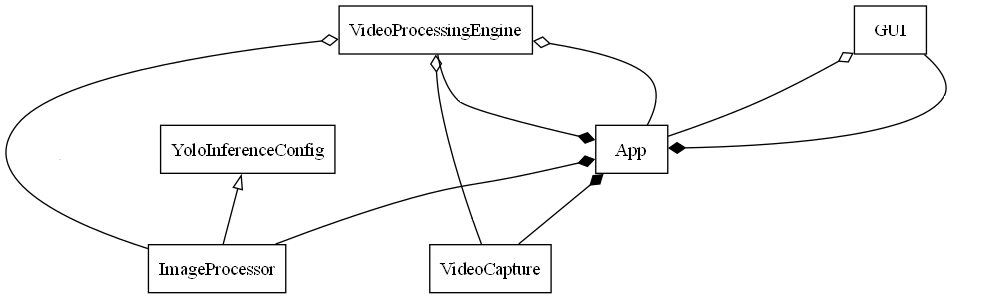
\includegraphics[width=\linewidth]{r_implementacja/klasy/simplified_classes.png}
    \caption{Uprosczony diagram klas UML (bez metod i pól) wygenerowany przez bilbiotekę \emph{pylint}.}
    \label{fig:uprosczony-diagram-klas}
\end{figure}

Tak jak wspomniano klasa \emph{YoloInferenceConfig} nie jest instancjowana -- programowe użycie jej pól odbywa się wewnątrz \emph{ImageProcessor}, zaś jej metody są wywoływane poprzez obiekt klasy \emph{ImageProcessor}. Jest to umożliwione dzięki dziedziczeniu \emph{YoloInferenceConfig} przez \emph{ImageProcessor}.

\emph{App} jako punkt startowy aplikacji tworzy w swoim konstruktorze obiekty klas \emph{VideoCapture}, \emph{ImageProcessor}, \emph{VideoProcessingEngine} oraz \emph{GUI}. Istnienie tych obiektów jest zależne od istnienia klasy App -- z perspektywy UML jest to kompozycja. Nazwy tych obiektów to według kolejności: \emph{\_image\_processor}, \emph{\_video\_capture}, \emph{\_video\_processing\_engine} oraz \emph{\_gui}. Następnie, plik główny programu (\emph{main.py}) wywołuję metodę \emph{run}. Metoda ta uruchamia silnik generacji klatek (\emph{self.\_video\_processing\_engine.run()}) oraz wyświetla graficzny interfejs użytkownika \emph{self.\_gui.show()}. Po zamknięciu GUI wykonywana jest ostatnia instrukcja -- wyłączająca silnik generacji klatek (\emph{self.\_video\_processing\_engine.shutdown()}). Opisane użycie zareprezentowano fragmentem kodu w listingu \ref{lst:app-instancjowanie}. 

\begin{lstlisting}[caption={Tworzenie obiektów klas wewnątrz \emph{App} oraz uruchomienie w niej różnych sekcji aplikacji.}, label={lst:app-instancjowanie}]
class App:
    # Konstruktor App
    def __init__(self) -> None:
        # ... reszta kodu
        # Tworzenie obiektow klas:
        self._video_capture = VideoCapture()
        self._image_processor = ImageProcessor()
        self._video_processing_engine = VideoProcessingEngine(self._video_capture, self._image_processor, self)
        self._gui = GUI(self)
        # reszta kodu ...

    # Metoda uruchamiajaca poszczegolne sekcje aplikacji
    def run(self) -> None:
        self._video_processing_engine.run()
        self._gui.show()
        self._video_processing_engine.shutdown()
\end{lstlisting}

Tak jak wspomniano w opisach klas, \emph{App} jest interfejsem komunikacyjnym między \emph{GUI}, a resztą klas potrzebnych \emph{GUI}. Do \emph{GUI} przekazywana jest referencja (obiekt) \emph{App}, z której poziomu utworzono obiekt \emph{GUI}. W celu pobrania bądź zmiany informacji w innych modułach \emph{GUI} wywołuje metody \emph{App} poprzez tę referencję. Z perspektywy \emph{GUI} jest to agregacja. Taki sam typ relacji dotyczy również \emph{VideoProcessingEngine} do \emph{App}, której referencje \emph{VideoProcessingEngine} wykorzystuje do wywołania metody alarmującej dźwiękowo użytkownika. Agregacja w \emph{VideoProcessingEngine} występuje również względem \emph{ImageProcessor} oraz \emph{VideoCapture}.


\section{Szczegóły implementacyjne}
W sekcji tej opisano implementacje wielowątkowego podejścia architektonicznego. Przedstawiono argumenty za wybraniem tego typu architektury, rozwiazanie problemów przez nią wywoływanych oraz uzasadnienie innych działań zastosowanych w celu poprawy wydajności systemu.  

Pierwsza iteracja oprogramowania była oparta na architekturze jednowątkowej. Sekwencyjnie wykonywano kolejne metody w nieskończonej pętli: pobór klatki z kamery, detekcja obiektów, alarmowanie dźwiękowe, wizualizacja obiektów oraz wyświetlenie klatki w wyświetlaczu graficznego interfejsu użytkownika.

Na tym etapie rodziału warto pochylić się nad działaniem modułu graficznego użytego w klasie \emph{GUI} --- tkinter. 
Jest on podstawą i jedyną wykorzystywaną technologią w implementacji panelu sterowania. Moduł ten dostarcza graficzne komponenty takie jak suwak, wykorzystany do zmiany progu ufności, przewijaną sekcja z polami wyboru wykrywanych klas obiektów, oraz menu do wyboru źródła wideo. 

Aby móc użytkować interfejs na bazie modułu, wymagane jest wywołanie głównej pętli tkinter (ang .\emph{mainloop}). Pętla opiera się ona na architekturze wydarzeniowej (ang. \emph{event-driven architecture}) działającej w ramach jednego, głównego wątku aplikacji. Poprzez wydarzenie rozumie się zdefiniowaną w module integrację z komponentem np. kliknięcie na przycisk. Zadaniem pętli jest zareagowanie na wydarzenia w sposób zfefiniowany przez moduł (np. wypełnienie przycisku kolorem po kliknięciu) oraz wykonanie kodu, który programista podłączył pod dane wydarzenia (np. wywołanie metody ustawiającej źródło wideo). Przykład na bazie kodu źródłowego pokazano w listingu \ref{lst:tkinter-event-loop}.


\begin{lstlisting}[caption={Podłączenie metod pod wydarzenia oraz zainicjalizowanie pętli głównej w module tkinter.}, label={lst:tkinter-event-loop}]
def GUI:
    # Metoda tworzaca panel sterowania
    def _initialize_control_panel(self) -> None:
        self._root = tk.Tk() # Utworzenie aplikacji (okna) tkinter
        # Utworzenie menu do wyboru zrodla wideo:
        self._menubar = tk.Menu(master=self._root)
        self._root.config(menu=self._menubar)
        self._initialize_video_source_menu()
        # reszta kodu metody ...

    # Metoda tworzaca menu z przyciskami do wyboru zrodla wideo 
    def _initialize_video_source_menu(self) -> None:
        self._source_menu = tk.Menu(master=self._menubar, tearoff=0)
        self._selected_video_source_id = tk.IntVar()

        sources = self._frame_generator.get_available_sources()
        for source_name in sources:
            # Stworzenie pojedynczego przycisku:
            self._source_menu.add_radiobutton(
                label=source_name,
                variable=self._selected_video_source_id,
                value=sources[source_name],
                # Podlaczenia zaprogramowanej funkcji do ustawienia zrodla wideo do wywolania po nacisnieciu przycisku:
                command=lambda source_index=sources[source_name]: self._on_video_source_select(source_index) 
            )

        self._selected_video_source_id.set(NO_VIDEO)
        self._menubar.add_cascade(menu=self._source_menu, label='Video source')

    # Metoda uruchamiajaca GUI (inizjalizuje petle tkinter)
    def show(self) -> None:
        # ... kod poprzedzajacy
        self._root.mainloop()
        # reszta kodu... (zostanie wykonana po zakonczeniu petli)

\end{lstlisting}

Z perpektywy programistycznej, instrukcje wywołane po instrukcji inicjalizacji zostaną wykonane dopiero po jej zakończeniu -- zamknięciu przez użytkownika okna aplikacji. Generuje to konieczność wywołania sekcji logicznej aplikacji przed rozpoczęciem pętli. Jest to jednak problematyczne, ponieważ sekcja ta musi stać się częścią mechanizmu tej pętli właśnie. Oferowanym rozwiązaniem jest funkcja również zawarta w tkinter -- \emph{after}. Funkcja ta przyjmuje liczbe całkowitą określającą czas w milisekundach, po którym zostanie wykonana metoda przekazana jako drugi argument tej funkcji. 

Użycie \emph{after} nie blokuje wykonania kolejnych instrukcji w kodzie dlatego też może być bezpiecznie użyte w ramach aplikacji tkinter. Zaprogramowanym sposobem użycia jest wywołanie metody do komunikacji z sekcją logiczną \emph{\_update\_frame}. Istotą tego rowiązania jest zawarcie w kodzie tej metody najpierw obsługi sekcji logicznej oraz późniejsze wywołanie tej samej metody przy użyciu funkcji \emph{after}. Nieblokujący mechanizm \emph{after} unika nieskończonej rekurencji prowadzącej do pojawienia się wyjątków pamięciowych systemu operacyjnego. Mechanizm wyświetlania przy użyciu opisanych funkcji opisano w listingu \ref{lst:tkinter-after}.

\begin{lstlisting}[caption={Wyświetlanie klatek obrazu w GUI przy pomocy modułu tkinter.}, label={lst:tkinter-after}]
AFTER_DELAY = 1 # Czas w milisekundach. Najmniejsze mozliwe ustawienie. 
class GUI:
    # Konstruktor klasy
    def __init__(self, communication_interface: App) -> None:
        # Ustawienie interfejsu do komunikacji z sekcja logiczna oprogramowania, w tym poboru klatek z kamery:
        self._communication_interface = communication_interface
        # reszta kodu ...

    # Metoda do uruchomienia GUI
    def show(self) -> None:
        self._root.mainloop() # inicjalizacja petli tkinter

    # Metoda uruchamiana w po ustawieniu kamery w panelu sterowania
    # Sluzy do rozpoczecia komunikacji z warstwa logiczna w celu poboru klatki do wyswietlenia  
    def _start_displaying(self) -> None:
        self._is_displaying = True
        cv.namedWindow('Display', cv.WINDOW_NORMAL) # Stworzenie okna wyswietlacza
        cv.moveWindow('Display', 0, 0)
        self._update_frame()

    # Metoda uruchamiana po zakonczeniu strumienia wideo
    # Sluzy zakonczeniu wyswietlania (zakonczenie poboru klatek)
    def _stop_displaying(self) -> None:
        self._is_displaying = False
        cv.destroyAllWindows() # Zniszczenie okna wyswietlacza

    def _update_frame(self) -> None:
        if not self._is_displaying:
            self._stop_displaying()
            return

        # Pobranie klatki (frame) oraz informacji o tym czy kamera dalej dziala (is_capture_on):
        is_capture_on, frame =  self._communication_interface.get_processed_frame()

        if is_capture_on:
            if frame is not None:
                self._show_frame(frame)
            # Jezeli kamera dziala, mechanizm kontunuowany:
            self._root.after(AFTER_DELAY, self._update_frame)
        else:
            self._frame_generator.set_video_source(NO_VIDEO)
            self._selected_video_source_id.set(NO_VIDEO)
            self._stop_displaying()

    # Metoda wywolywana do wyswietlania klatki obrazu
    def _show_frame(self, frame: MatLike) -> None:
        frame = cv.cvtColor(frame, cv.COLOR_BGR2RGB)
        cv.imshow('Display', frame) # Wyswietlenie klatki
\end{lstlisting}

Użycie interfejsu w celu pobrania klatki (\emph{self.\_communication\_interface.get\_processed\_frame()}) pozwoliło oddzielić sposób pozyskania klatki od architektury komunikacyjnej między sekcją GUI, a sekcją logiczną oraz zachować taki sam kod klasy \emph{GUI} dla następnych iteracji systemu. W przypadku iteracji jednowątkowej użycie metody interfejsu wywoływało następującą sekwencję kroków: pobór klatki z kamery; zmniejszenie rozmiaru klatki, tak aby zmieściła się na ekranie komputera; detekcja obiektów; alarmowanie dźwiękowe oraz wizualizacja prostokątów ograniczających w przypadku wykrycia obiektów; zwrócenie przetworzonej klatki obrazu.

Długa sekwencja zadań oraz czasochłonność niektórych operacji (np. detekcji obiektów) blokowała odświeżanie oraz dostęp do funkcji komponentów GUI, czyniąc go oraz cały system nieresposywnym i powolnym. W celu poprawy optymalizacji nie zdecydowano się zmienić ustawionego, minimalnego czasu, po którym następują kolejne wykonania \emph{\_update\_frame}, ponieważ ryzykowano by utratą wiekszej ilości pobieranych klatek -- kluczowych dla alarmowania użytkownika -- pomimo poprawy responsywności interfejsu graficznego.

Pierwszym podjętym krokiem w celu poprawy wersji jednowątkowej było przeniesienie wykonania inferencji (detekcji) z CPU na GPU. Parametr do tego użyty był opisany w rodziale \ref{chap:wprowadzenie-yolo_interjes}. Poprawiło tym znacznie wydajność uzyskania finalnej klatki, aczkolwiek GUI nadal borykało się z problemem responsywności. Postanowiono więc zmienić architekturę na wielowątkową. Podejściem takim osiągniąto zamierzone rezultaty -- GUI osiągneło zadowalający poziom responsywności przy zachowaniu satysfakcjonującej wydajności (opisanej w rozdziale \ref{chap:test-szybkosci}, testów szybkości systemu). 


